\section{VideoGPT}

\begin{figure}
    \centering
    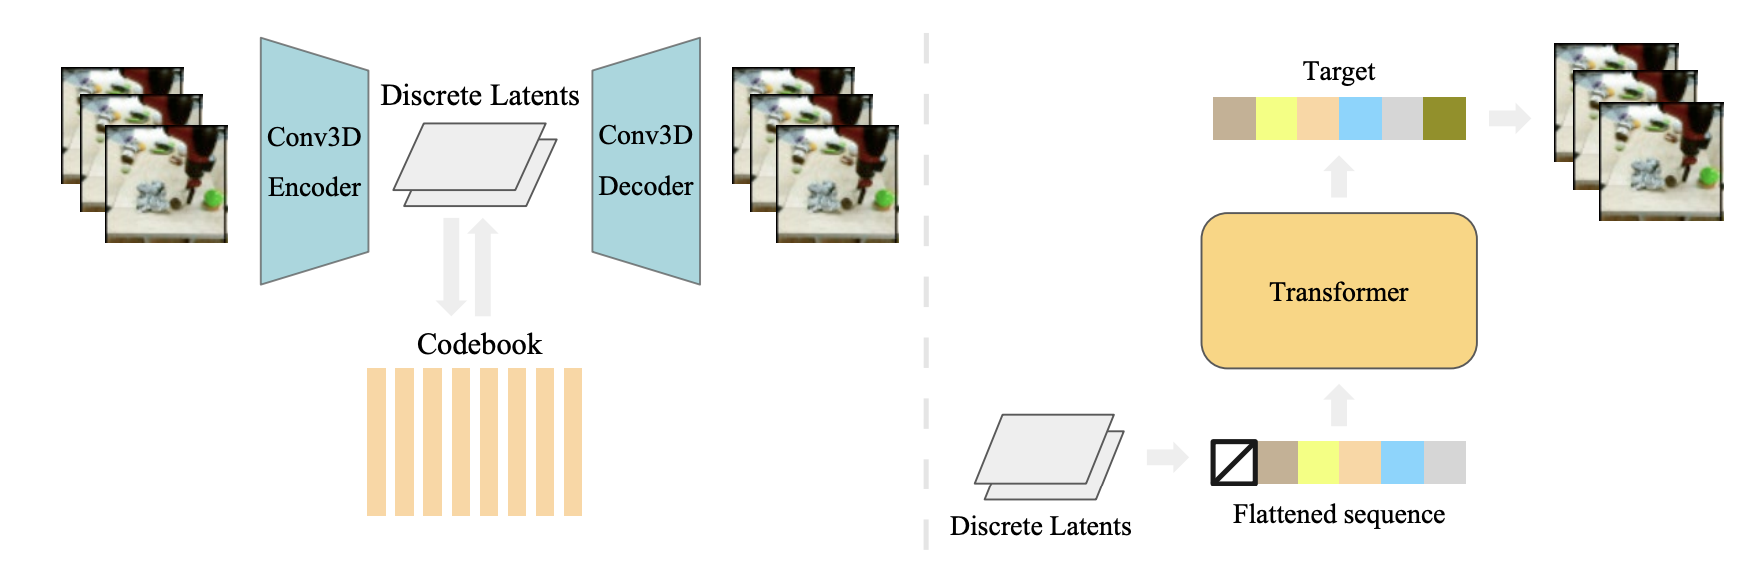
\includegraphics[width=0.7\textwidth]{images/video_synthesis/videogpt_architecture.png}
    \caption{VideoGPT architecture. Left: training the VQ-VAE; Right: training the autoregressive transformer model on the latent vectors.}
\end{figure}

\begin{figure}
    \centering
    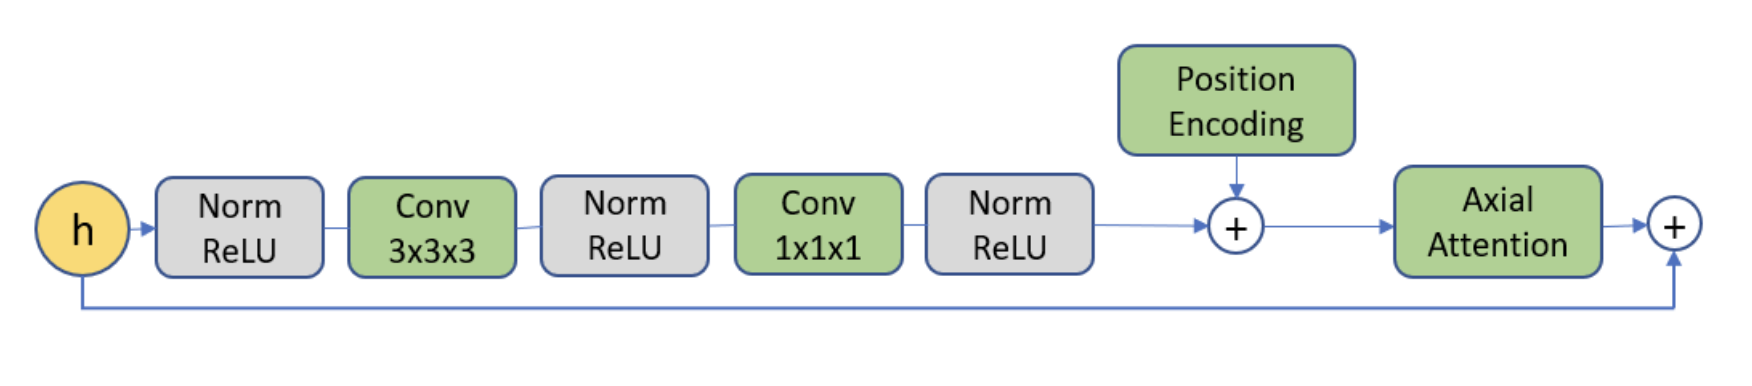
\includegraphics[width=0.6\textwidth]{images/video_synthesis/videogpt_res_atten_block.png}
    \caption{Residual attention block as described in VideoGPT. The "Norm" layers are \texttt{LayerNorm} blocks (described in appendix \ref{appendix:blocks_norm}).}
    \label{fig:videogpt_res_atten_block}
\end{figure}

VideoGPT \cite{videogpt} uses likelihood based model VQ-VAE and GPT-like transformer model. The encoder of VQ-VAE first downsamples video into discrete latent space using 3D convolutions, and the decoder then reconstructs the video from these latent codes (by using a codebook - see VQ-VAE section \ref{sec:vqvae}). The generated latents are decoded to the original video resolution as the training dataset.

The researchers take inspiration from image and video codecs: JPEG and MPEG for image and video compression. They contain the same spatio-temporal data as the uncompressed video, yet take less resources (by not working in the pixel space).

Reminder that the loss function of VQ-VAE is defined:

\begin{equation*}
    \mathcal{L} = \underbrace{\left| \left| x - D(e) \right| \right|^2_2}_{\mathcal{L}_\text{recon}} + \underbrace{\left| \left| \text{sg}\left[ E(x) \right] - e \right| \right|^2_2}_{\mathcal{L}_\text{codebook}} + \underbrace{\beta \left| \left| \text{sg}[e] - E(x) \right| \right|^2_2}_{\mathcal{L}_\text{commit}}
\end{equation*}

where $\text{sg}$ refers to stop-gradient, $\mathcal{L}_\text{recon}$ is the reconstruction loss (mean squared error), $\mathcal{L}_\text{codebook}$ is the codebook loss (quantization loss), and $\mathcal{L}_\text{commit}$ is the commitment loss. The decoder optimizes the reconstruction loss only, the encoder optimizes the commitment loss only, and the codebook embeddings are optimized in the codebook loss (depending on the stop-gradient). See section \ref{sec:vqvae} for more details.

The researchers used EMA update \cite{vqvae} for the codebook loss which is a (exponential) moving average of the codebook embeddings. In short, it makes the VQ-VAE faster to train and faster convergence speed.

As described in section \ref{sec:vqgan}, GPT is autoregressive transformer model. The autoregressive nature can be described as $p(x) = \prod_{i=1}^{d} p(x_i | x_{\leq i})$ through masked self-attention.






\subsection{Architecture}

They train the VQ-VAE on video data to learn the codebook. The encoder and decoder consists of 3D convolutions (appendix \ref{appendix:blocks_3dconv}) followed by attention residual blocks (figure \ref{fig:videogpt_res_atten_block}). Axial attention block is described in appendix \ref{appendix:blocks_axial_attention}.